\section{Condition monitoring}
All rotating machinery eventually fail because of the long-term strain on the individual parts or incorrent workmanship, installation or operational procedures. In the end, these factors cause the equipment not to fulfill its intended functionality. Many instrumentation methods are practiced to reveal evolving faults: vibration and acoustic noise monitoring, electric supply line measurements, thermography, wear debris analysis, ultrasonic testing, etc. Vibration signals are the preferred tool for rotating machinery monitoring \cite{mohanty_machinery_2015}. 

The defect needs to be either repaired or replaced, preferably without significant production downtime, futher damage to the other attached elements or endangerment of the responsible personnel. The maintenance strategies are chosen according to the machine's importance as a result of its failure effect evaluation on the system. The guide to set appropriate maintenance procedures is outlined by IEC 60706-2 standard and involves reliability-centered maintenance (RCM) analysis \cite{el-thalji_predictive_2019}.

\subsection{Maintenance strategies}
There are three different approaches to maintenance across the industry: reactive, preventive, and predictive \cite{scheffer_practical_2004}. In general, the more sophisticated methods are beneficial in a high stakes environment. The unexpected machine shutdown can have negative economic impact on the enterprise, resulting in the decreased product quality and demands spare parts be ready in the supply inventory at all times. However, in certain situations suffice to utilize a simpler maintenance program, but predictive maintenance is gains interest in the Industry 4.0 to optimize usage of assets \cite{cinar_machine_2020}.

\paragraph{Reactive maintenance} allows machinery to run to complete failure. This is the most inefficient way to maintain production line. It requires large stock of replacement parts on site and breakage constitutes a ,,crisis management mode'' in the plant \cite{scheffer_practical_2004}. On demand repairs are justified for consumer products or in the factory capable to fully and quickly replace halted machine with a backup. 

\paragraph{Preventive maintenance} is performed before any issue is detected. Maintenance occurs at regular intervals derived from a predetermined period in the calendar or expected machine running time (e.g. MTTF - Mean Time To Failure). The schedule is crucial but can result in components being replaced in good condition when further utilization is possible or too late after the machine breaks. In this case, conservative planning is usually the norm which means more frequent intervention \cite{mohanty_machinery_2015}.  


\paragraph{Predictive maintenance} known as condition-based (CbM), improves the predictibility of reactive maintanace and eliminates the waste in overall resource utilization of cautious prevention. The machine downtime is scheduled after the detection of unhealthy trends in fault monitoring and troublesome components are identified. This allows to order necessary parts in advance and organize repairs of several machines at a convinient time. The misdetection leads to increased costs compared to previous methods and raises the expectation that faults are distinguishable among themselves. \cite{davies_handbook_2012}.

\subsection{Diagnosis indicators}
\begin{figure}[h]
\centering
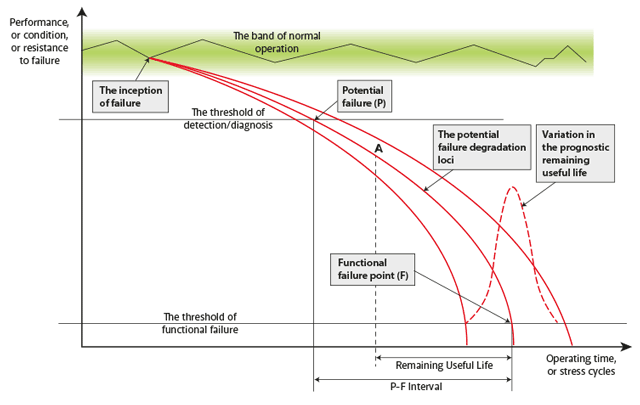
\includegraphics[width=\textwidth]{assets/P-F-Curve.png}
\caption{P-F curve \cite{jennions_integrated_2011}}
\end{figure}

- what we montitor? - when it fails and early signs of faulty component
- P-F Curve  = Wear process curve (Bathtub curve), 
- RUL (Remaining useful life) models - disadvantage lot of similiar machines (homogenous) or lots of runns until failure
% Overview of Remaining Useful Life Prediction Techniques in Through-Life Engineering Services
\cite{okoh_overview_2014}
\begin{itemize}
\item Survival (Analytical-Based)
\item Similarity (Model-based)
\item Degradation - used by standards (Knowledge-Based)
\end{itemize}

\subsection{Vibration fault types}
Why monitor with vibrations,
- frequency ranges 1 - 300 Hz (shaft), 300 - 1000 Hz, 1000 - 10000 Hz (early bearings)
- Base analytical models: Jeffcott rotor - rotor dynamics, Bearnings model
- Resonance frequencies of each part - machine must run at speeds not aligned with resonance frequencies - Campbell diagram - task for mechanical engineers
- Faults - reasons and frequency content
% Automatic Anomaly Detection in Vibration Analysis Based on Machine Learning Algorithms
\cite{torres_automatic_2022}
% Vibration Guide
\cite{noauthor_vibration_2000}
% The experimental application of popular machine learning algorithms on predictive maintenance and the design of IIoT based condition monitoring system
\cite{cakir_experimental_2021}
% Technická diagnostika
\cite{ziaran_technicka_2013}

\begin{itemize}
\item Synchrounous response - based on RPM
\item Mass unbalance
\item Misalignment
\item Eccentricity
\item Bent or bow shaft
\item Cracked shaft
\item Rotor rubs - friction
\item Looseness
\item Auxiliery mechanical systems: Gearbox, Bearings, Belt 
\end{itemize}

% Bandsaws
% Vibration of bandsaws
\cite{lengoc_vibration_1990}
% Study on Online Detection and Fault Diagnosis of Band Saw Equipment
\cite{chen_study_2014}

\subsection{Technical standards}
\paragraph{ISO 20816}
% ISO 20816-1:2016 - Mechanical vibration - Measurement and evaluation of machine vibration - Part 1: General guidelines
\cite{noauthor_iso_2016}
Part 1
\begin{itemize}
\item Measurement units - displacement, velocity, acceleration
\item RMS, and max. amplitude = severity
\item Measurement points for sensors (axial, radial) - image, and 45 degrees
\item Evaluation zones - A, B, C, D - Severity chart (Annex B) - Degradation model
\item Opeartional limits - Alarm, Trips
\end{itemize}

\paragraph{ISO 13373}
% ISO 13373-1:2002 - Condition monitoring and diagnostics of machines - Vibration condition monitoring - Part 1: General procedures
\cite{noauthor_iso_2016}
% ISO 13373-2:2016 - Condition monitoring and diagnostics of machines - Vibration condition monitoring - Part 2: Processing, analysis and presentation of vibration data
\cite{noauthor_iso_2016-1}

\cite{jack_d_frequency_nodate}
\begin{itemize}
\item Sensor mount type in relation to sensor resonance
\item Data presentation - standard display formats for analysis - trends, watefall plots ...
\item Potencial causes for faults (p. 45) - use in vibration fault types
\end{itemize}
 
